% Discuss the DOE project and how it is relevant

\chapter{Smart Grid and Smart Meters}
\label{chapter:doe}

\section{Overview}
There has been a move recently towards the design and implementation of what is called a "smart grid." A smart
grid is an electrical power grid which can gather information about the meters, houses, and consumers of
electricity that are attached to it.


By gathering information from a smart grid, a power company can more efficiently manage its production and delivery
of electricity, thus reducing cost. Not only does the smart grid help the power company, but by providing analytics to
its customers, customers can adjust their consumption habits to lower their bills as well. With the increasing cost of
fossil fuels and the increasing energy consumption of today's consumer, reducing wasted electricity will be very useful.

Naturally, with this increase in functionality, there is an increase of risk as well. While the power company can use
the smart grid to smartly redirect power to where it is needed, an attacker might try to direct power away from an
area or direct so much power to an area that the system becomes overloaded and fails.

As a response to the increased dangers that a smart grid provides, we describe a system that is designed to allow
for secure, yet convenient, communication and management between consumers and the utility company. Existing
systems are leveraged, such as the ZigBee mesh network~\cite{zigbee}, which is further described below.
One of the main things that is critical in this new system is that individual meters are able to be uniquely identified
so billing can be done correctly, but also so no one can impersonate them. This is a perfect opportunity for PUF
technology.

\section{Actors}
For the rest of the chapter, it will be useful to discuss the different players in the smart grid scenario.

\subsection{Utility Company}
One of the major players in the smart grid scenario is the utility company. The utility company is responsible for
generation of the electricity using techniques such as coal power, hydroelectric, wind, among others. The utility
company is also responsible for managing the dynamic delivery of power to areas that need it.

Finally, the utility company is also responsible for maintaining information on all of its customers and billing them
appropriately.

\subsection{Substations}
Substations receive large amounts of high voltage power from the utility company. However, this power is not ready
for end user consumption. The substation thus takes the power from and converts it to  more reasonable levels
that is suitable for being to delivered to end users.

The substation will communicate with the utility company to tell the utility how much load it is under. Depending on
the load, it will then receive more or less power. It also acts as a sort of "collector" node for different smart meters.
Smart meters will communicate with the substation which will then relay the data back to the utility company.

\subsection{Smart Meters}
A smart meter is much like a regular power meter but with some added features. Smart meters measure power as
a normal meter, but they can typically be configured so that they can also "rewind" if a user is pumping power back
into the grid. Additionally, smart meters have many different features which allow real time information and analytics
about power consumption to be obtained.

One of the large benefits of smart meters is that the utility company can communicate and read them without
necessarily sending a worker out to read the values. This is much faster and more cost effective than traditional
power meters. This is accomplished using some sort of wireless interface. Typically, the ZigBee~\cite{zigbee}
~\cite{aminetworking}
wireless protocol is used and is set up so that all meters form a mesh network with each other. This allows meters
that are not within wireless range of a substation (or some other communication center) to still talk to the substation.
This is accomplished since each smart meter not only transmits its own data, but it also acts as a relay for other nodes
in the mesh network.

Note that smart meters have some amount of general purpose computation, but they are not very powerful. As such,
it is necessary to optimize programs so that they can be run on the smart meters.

The smart meters used in this project are produced by Landis+Gyr. They consist of two components of interest. One
board is called the "metering board" and is responsible for measuring and recording information about the actual
power consumption of attached devices. The other board is called the "communication board". It is responsible for
performing the different types of communication as necessary. The two are connected over an event-based interface,
but this interface is not encrypted. 

There are 5 security levels on the smart meter, each giving a different amount of privilege to different meter controls,
with level 0 being read only access and level 5 giving control of everything. There is a table in the smart meter which
stores each of the corresponding keys for the levels; These keys are referred to as access level keys.
Communication between the utility and smart meter is encrypted
using a random session key, which is derived from an encryption key.

\section{Physical Systems}
The actors above are clearly examples of physical systems. All three heavily interact with the environment around them
to fulfill the power needs of consumers.

The utility company as a whole might not be considered a physical system, but parts of it will definitely be considered
examples of deployed physical systems. The utility must manage the production of electricity by its generators as well
as well as manage the communication of commands to the various smart meters, via the mesh network.

Substations could also be considered deployed physical systems, since they perform a large amount of interaction
with the physical world to transform the power from the utility company into power that is usable by consumers.
They additionally must take a large amount of input from both consumer smart meters and the utility to decide how
to manage the power resources in a dynamic way.

The smart meters are deployed physical systems. A large part of the smart meters job is to record and analyze
the power usage of the home or building they are attached to. This requires interaction with the physical world. However,
smart meters are also clearly networked, since they can have so much interaction across them (in the 
concept of the mesh network) and the utility company.

\section{Protocol}
Our goal is to provide a protocol that allows for secure, authenticated communication between the utility company and
smart meters, in the presence of and despite different types of adversaries.
We leverage the use of a PUF device in conjunction with the smart meter to uniquely identify the smart meter to the
utility company.

Before describing the protocol itself, it will be helpful to discuss the information each party is expected to maintain.
The utility company will maintain a database containing two tables, one for zero knowledge commitments and the 
other for 
access level keys. The first table, referred to as the authentication table, will correlate a specific meter with a zero knowledge proof.
The second table, referred to as the access level key table, will correlate a smart meter with the five keys for the five different security levels of the 
meter. This table also stores the encryption key.

The smart meter needs to store the public key of the utility company and also maintain a "master key"
that is generated internally using the PUF. 

Both parties also need enough information about
the mesh network to ensure that they can communicate with each other. Both parties also need to share the
encryption key, which is used to derive temporary session keys.

The first step that must be done is that the utility company must record a zero-knowledge commitment from the 
smart meter for a specific challenge. This is illustrated in Figure~\ref{fig:doeconfig}. This step is required so that later
in the protocol, the smart meter can execute a zero-knowledge proof to prove its identity.
Note that this step must be done out-of-band from the mesh network, lest an adversary enter an invalid commitment.
This could be done at manufacture time or at installation time by a technician, as long as it is executed through a secure channel.

\begin{figure}[!ht]
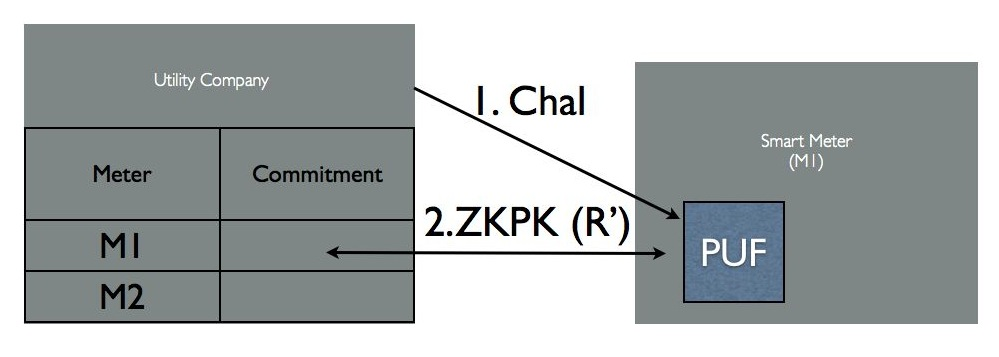
\includegraphics[width=400px]{images/doe_auth_config.jpg}
\caption{Enrollment of the Commitment}
\label{fig:doeconfig}
\end{figure}
\FloatBarrier

After the commitment phase has been completed and the meter has been deployed, the \textit{keying} operation
can be performed. This operation starts by executing a key derivation protocol. Recall that the smart meter 
maintains a "master key" which is generated by the PUF. 
This master key is passed through some sort of one-way function, such as a hash
in the style of $K_1=H(MK|1), K_2=H(MK|2)...$ so that six new keys are derived, but the original master key is
never revealed. These six keys are then
encrypted under the public key of the utility company. All the encrypted keys as well as a zero knowledge proof
are then sent to the utility company. The ZKPK allows the utility company to authenticate the encrypted keys before
updating its database with the six new entries. This transmission step is detailed graphically in~\ref{fig:doeusage}.
Figure~\ref{fig:keyderivation} graphically describes the key derivation process.

Note that the PUF uses an internal feedback loop, so that every invocation of the keying procedure will generate a
different PUF response, which will in turn generate different derived keys.

\begin{figure}[!ht]
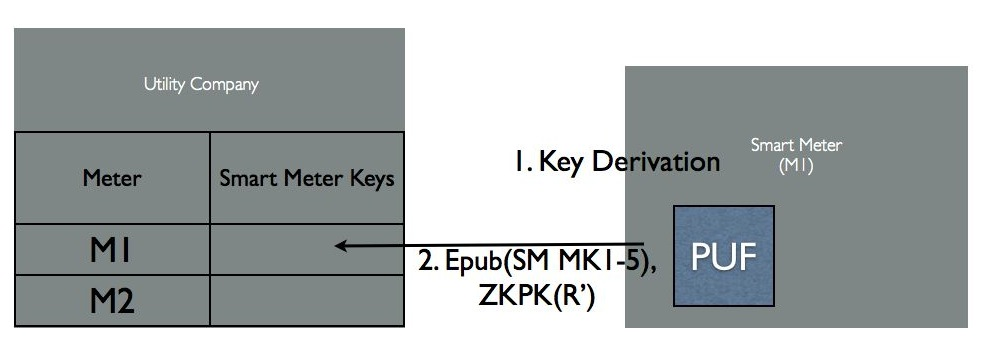
\includegraphics[width=400px]{images/doe_key_config.jpg}
\caption{Storage of the Derived Keys}
\label{fig:doeusage}
\end{figure}
\FloatBarrier

\begin{figure}[!ht]
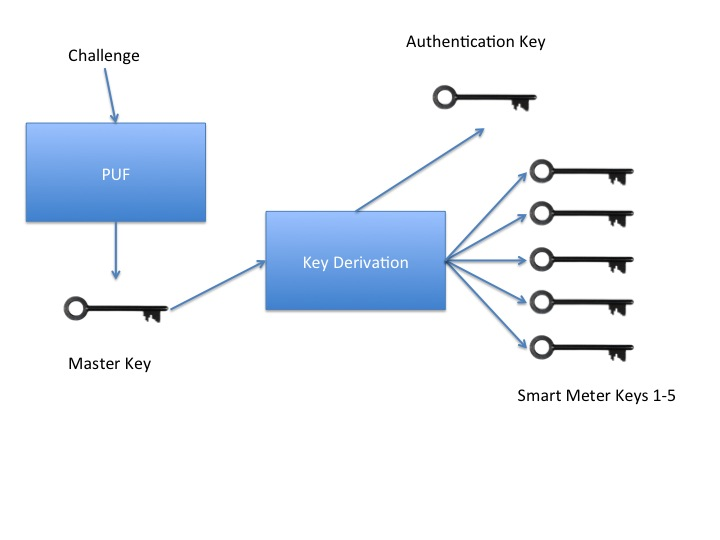
\includegraphics[width=400px]{images/keyderivation.jpg}
\caption{The Key Derivation Process}
\label{fig:keyderivation}
\end{figure}
\FloatBarrier


After the utility company has received these five access level keys and the encryption key, 
interactions between the smart meter and the utility company
will then proceed as it currently does. That is, the smart meter and utility company will use the shared encryption
key to compute a temporary, symmetric session key which will be used to encrypt data that is sent between the two.

Note that since the smart meter has limited computation powers, the operations above are fairly expensive. This
is acceptable though, since the enrollment and keying operations will be done very infrequently. If they need to
be re-run, this can be planned ahead for off peak times, such as in early morning and consumers can be notified
of this. The symmetric session key is frequently used, but symmetric encryption is much less computationally expensive
than asymmetric encryption.

Additionally, note that the utility company signs any correspondence during the enrollment or keying stages.
This allows the smart meter to validate the signature and thus ensure that commands are actually coming
from the utility company.

\section{Security Considerations}
Because there are several different ways in which the system could be compromised and the gravity that
such a compromise could have, it is necessary to consider and discuss the different security issues. 

Note that a distinction is made between the set of initial enrollment and keying operations that we defined versus
the existing system of encryption using session keys.

\subsection{Meshnet Transmission Security}
% Discuss how we use application level security, not just the ZigBee and other protocols
One potential problem is that when data is being transmitted across the meshnet, rather than relaying, a node
may attempt to read the data in transit. This would be considered a man in the middle attack. There are encryption
layers imposed by the ZigBee protocol and other transmission protocols, but it stands to reason that if a node were
malicious, it might be able to crack these layers.

As such, we add another layer of security at the application layer. Data is encrypted under the public key of the utility
company during the keying operation. As such, an adversary would be required to compromise the public key
algorithm, which is considered computationally unfeasible. A more likely attack would be to compromise the private key
of the utility company. This possibility is considered separately below.

Data being transmitted using the session key between the utility company and smart meter is encrypted under a
symmetric key algorithm, EAX', which is a variant of AES that is defined under ANSI standard 
C12.22~\cite{ansi1222}~\cite{eax}. As such, an adversary would have to be able to defeat this algorithm to make
any progress. An attack on EAX' has been reported~\cite{eaxflaw}, but this attack is new and may not be effective
enough to compromise the total integrity of the communication.

The system is also resilient against replay attacks in this situation, since both time stamps and nonces are incorporated.
As such, any replay will have invalid time stamps and nonces, so will not be valid.

There is a risk of a denial of service if an active adversary simply drops all traffic, but this is considered an acceptable
risk.

\subsection{Compromised Smart Meter Key or Encryption Key Compromise}
It is possible that somehow, one of the five smart meter keys or the encryption key used to derive session keys
could be compromised. This might happen if an employee copies a key from the database or for any other number
of reasons. Even if this happens, security is only temporarily effected.

Recall that the master key generated from the PUF is passed through a one way, key derivation process. As such,
even if one of the derived keys (the smart meter keys or the authentication key) is compromised, the master key
is still secure. To re-secure the system, the keying procedure will then be re-run, which will provide a brand new set
of smart meter keys and authentication key.

This procedure is essentially analogous to a re-key request, even if there is no compromise.

Note that this case is separate from the databases containing this information, which is considered below.

\subsection{Utility Database Compromise - Commitment Table}
If the commitment table in the utility database is compromised, the results will not be catastrophic. Since the committed
values for the ZKPK do not leak any information, the adversary will not be able to impersonate any users or garner
any new information about the underlying authentication key.

The worst case is when the adversary changes the committed values in the database. This would essentially create a
denial of service attack. However, he could also update the database with his own commitment value and place
himself between the smart meter and the utility company as an active MITM and then impersonate the smart
meter. 

Since he would be able to authenticate to the utility server, he could thus send false data about consumption or 
whatever he wanted. This threat could be dealt with by making sure that the database is very secure
and that the entries are  carefully monitored and updates are only allowed during the keying operation.

Note that in this case, the adversary would not be able to impersonate the utility company to the smart meter,
since he would not know the private key of the utility, which is necessary to sign the various messages.

This compromise would have no effect on the messages being sent under the temporary session key, since
there is no need for the authentication key during that stage.

\subsection{Utility Database Compromise - Key Tables }
It is possible that the database storing the smart meter access level keys or encryption key could be compromised. 
If these keys were compromised, the adversary could then access the sensitive commands
of the smart meter or read the interim traffic between the two parties.

However, this is not necessarily a real danger, since the keys are encrypted under the utility's private key before being
stored into the database. As such, the adversary would only recover ciphertext. Assuming he cannot break the public
key algorithm, the data will remain secure.

There is a possibility that if the database was compromised, the adversary might have been able to recover a key
as it is being decrypted in memory and record that. As such, it is wise to execute a re-keying operation for any meters
whose information was stored in that database.

\subsection{Utility Company Private Key Compromise}
One of the worst case scenarios is that the private key of the utility would become compromised. As previously
described, the smart meter's PUF-derived master key would remain secure, since it is never transmitted.

However, all smart meter access level keys and encryption keys could potentially be compromised, since the adversary
would record all traffic during the keying operation and use the private key to recover the keys.

Once those keys were recovered, it would be trivial for the adversary to communicate with the smart meter to
execute sensitive commands, request re-key operations, or whatever the adversary desired.

To recover from this attack, the old private key would first need to be discarded. Following that, the new public key would
need to be installed in every single meter in the grid. This would have to be done by hand, since any network
transmissions could not be trusted. Additionally, every smart meter would then need to execute the keying operation
so that the utility company could then update its database with the new values.

These recovery procedures would be very expensive and time consuming. As such, it is critical that the private key
never becomes compromised. Key management is a difficult, open problem that needs to be solved.

\subsection{Smart Meter Physical Security}
Since smart meters are physical systems, it is necessary to discuss and consider some of the physical threats they face.

The smart meters are actually designed to be fairly tamper resistant. If the external glass shell is removed without the
use of a technician's key, a signal is sent over the network to alert the utility company. After that happens, the utility
company can then flag any future traffic as suspicious and send a technician out to investigate and fix the meter.
Regardless, improving the tamper resistance of smart meters would be a good step to take.

Because the smart meter is doing cryptographic operations, it could potentially be vulnerable to power analysis
attacks as well as monitoring of emitted signals. To resolve this, some sort of potting mechanism, power filtering,
and shielding should be implemented. 

As previously described, the PUF is extremely resilient against tampering, so it will likely not be a problem.
Incorporating all the different components on a system on chip will be a good step towards security, since this will
hide all the internal buses as well as protect the areas with sensitive information stored on them.

\section{Implementation}
For the proposed scenario and protocol, we developed a proof of concept implementation. In the interest of time and
difficulty, rather than creating an entire smart meter from scratch, we opted to implement the 
PUF inside an FPGA and perform some of the network communication and computations on a PC, the smart meter
PC, which was connected to another PC, which is modeling the utility company. The smart meter PC is connected
to an actual smart meter via an optical port. The smart meter is also connected to the utility PC via a ZigBee interface,
as would be used in the actual field. Figure~\ref{fig:doeimpl} represents the prototype architecture.

\begin{figure}[!ht]
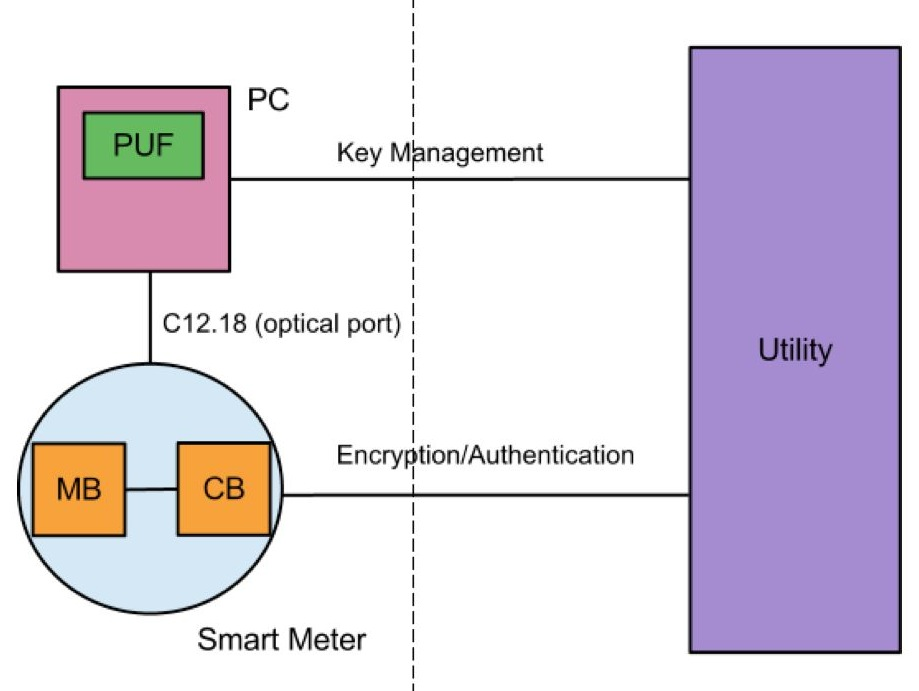
\includegraphics[width=400px]{images/doe_impl.jpg}
\caption{Prototype Implementation of Smart Grid Project}
\label{fig:doeimpl}
\end{figure}
\FloatBarrier

We used the Xilinx Spartan-6 Embedded Development board for our FPGA platform. This board was useful since we 
were able to incorporate an existing PUF design on it. Additionally, we were able to use the Microblaze soft core
microprocessor which Xilinx provides. As mentioned in Chapter~\ref{chapter:pear} and Chapter~\ref{chapter:rok},
it is a good idea to include the microprocessor on the same chip as the PUF device. This allows buses sending
sensitive information, such as PUF responses, to be better protected against adversaries. Again, inserting logic
probes into the inner parts of the chip would most likely disrupt the PUF, so any results obtained about the PUF would
thus be useless.

For the smart meter PC, we created an application in C++ which uses standard networking libraries to communicate
with the utility PC. The smart meter PC interacts with the PUF board via a serial port connection. The PC also contains
drivers and code to communicate with the actual smart meter over an optical port interface.

\subsection{Limitations}
Our approach has many different components that are not necessarily going to be present in an actual, deployed
system. For instance, the fact that the PUF board and the smart meter PC are separate from the smart meter is
a major issue that would not work in the field. 

In the future, it would be better to integrate all the control circuitry,
PUF device, and metering circuitry into a single chip, such as a large FPGA or even an ASIC design. In this way, only
one chip would need to be installed into the smart meter, rather than the large amount of devices currently needed.
